\documentclass[../main.tex]{subfiles}

\begin{document}

\chapter{Programming with MATLAB}

\label{cha:cha3}


\begin{center}
\Large{\textbf{CHAPTER OBJECTIVES}}
\end{center}

\normalsize{The primary objective of this chapter is to learn how to write M-file programs to
implement numerical methods. Specific objectives and topics covered are}
'
\begin{itemize}

    \item Learning how to create well-documented M-files in the edit window and invoke
    them from the command window.
    \item Understanding how script and function files differ.
    \item Understanding how to incorporate help comments in functions.
    \item Knowing how to set up M-files so that they interactively prompt users for
    information and display results in the command window.
    \item Understanding the role of subfunctions and how they are accessed.
    \item Knowing how to create and retrieve data files.
    \item Learning how to write clear and well-documented M-files by employing
    structured programming constructs to implement logic and repetition.
    \item Recognizing the difference between \texttt{if$\ldots$elseif} and \texttt{switch} constructs.
    \item Recognizing the difference between \texttt{for$\ldots$end} and \texttt{while} structures.
    \item Knowing how to animate MATLAB plots.
    \item Understanding what is meant by vectorization and why it is beneficial.
    \item Understanding how anonymous functions can be employed to pass functions to
    function function M-files.

	\item Learning how real and complex numbers are assigned to variables
	\item  Learning how vectors and matrices are assigned values using simple assignment,
the colon operator, and the linspace and logspace functions.
\item  Understanding the priority rules for constructing mathematical expressions.
\item  Gaining a general understanding of built-in functions and how you can learn more
about them with MATLAB's Help facilities.
\item  Learning how to use vectors to create a simple line plot based on an equation.
\end{itemize}
\bigskip
\bigskip
\Large{YOU'VE GOT A PROBLEM}
\normalsize

n Chap. 1, we used a force balance to develop a mathematical model to predict the
fall velocity of a bungee jumper. This model took the form of the following differential
equation:

$$\dfrac{dv}{dt}=g-\dfrac{c_d}{m}v|v| $$

We also learned that a numerical solution of this equation could be obtained with Euler's
method:
$$v_{i+1} = v_i +\dfrac{dv_i}{dt}\Delta t$$

This equation can be implemented repeatedly to compute velocity as a function of
time. However, to obtain good accuracy, many small steps must be taken. This would be
extremely laborious and time consuming to implement by hand. However, with the aid of
MATLAB, such calculations can be performed easily.

So our problem now is to figure out how to do this. This chapter will introduce you to
how MATLAB M-files can be used to obtain such solutions.

\section{M-FILES}

The most common way to operate MATLAB is by entering commands one at a time in the
command window. M-files provide an alternative way of performing operations that
greatly expand MATLAB's problem-solving capabilities. An M-file consists of a series of
statements that can be run all at once. Note that the nomenclature "M-file" comes from the
fact that such files are stored with a texttt{.m} extension. M-files come in two flavors: script files
and function files.

\subsection{ Script Files}

A $script$ file is merely a series of MATLAB commands that are saved on a file. They are
useful for retaining a series of commands that you want to execute on more than one occasion. The 
script can be executed by typing the file name in the command window or by
invoking the menu selections in the edit window: \textbf{Debug, Run}.

\section*{EXAMPLE 3.1 Script File}

roblem Statement. Develop a script file to compute the velocity of the free-falling
bungee jumper for the case where the initial velocity is zero.


Solution. Open the editor with the menu selection: \textbf{File, New, M-file}. Type in the following statements to compute
 the velocity of the free-falling bungee jumper at a specific time
[recall Eq. (1.9)]:

\begin{lstlisting}[frame=none, numbers=none]
    g = 9.81; m = 68.1; t = 12; cd = 0.25;
    v = sqrt(g * m / cd) * tanh(sqrt(g * cd / m) * t)
\end{lstlisting}



Save the file as scriptdemo.m. Return to the command window and type
\begin{lstlisting}[frame=none, numbers=none]
    >>scriptdemo
\end{lstlisting}
The result will be displayed as
\begin{lstlisting}[frame=none, numbers=none]
    v =
        50.6175
\end{lstlisting}
Thus, the script executes just as if you had typed each of its lines in the command window.


As a final step, determine the value of g by typing
\begin{lstlisting}[frame=none, numbers=none]
    >> g
    g =
         9.8100
\end{lstlisting}

So you can see that even though g was defined within the script, it retains its value back in
the command workspace. As we will see in the following section, this is an important distinction between scripts and functions.

\subsection{ Function Files}


$Function$ files are M-files that start with the word \texttt{function}. In contrast to script files, they
can accept input arguments and return outputs. Hence they are analogous to user-defined
functions in programming languages such as Fortran, Visual Basic or C.
The syntax for the function file can be represented generally as
\begin{lstlisting}[frame=none, numbers=none]
    function outvar = funcname(arglist)
    % helpcomments
    statements
    outvar = value;
\end{lstlisting}

where \texttt{outvar} = the name of the output variable, \texttt{funcname} = the function's name,
\texttt{arglist} = the function's argument list (i.e., comma-delimited values that are passed into
the function), \texttt{helpcomments} = text that provides the user with information regarding the
function (these can be invoked by typing {Help funcname} in the command window), and
\texttt{statements} = MATLAB statements that compute the\texttt{ value} that is assigned to \texttt{outvar}.
Beyond its role in describing the function, the first line of the \texttt{helpcomments}, called
the H1 line, is the line that is searched by the \texttt{lookfor} command (recall Sec. 2.6). Thus,
you should include key descriptive words related to the file on this line.
The M-file should be saved as \texttt{funcname.m.} The function can then be run by typing
\texttt{funcname} in the command window as illustrated in the following example. Note that even
though MATLAB is case-sensitive, your computer's operating system may not be.
Whereas MATLAB would treat function names like \texttt{freefall} and \texttt{FreeFall} as two different variables, your operating system might not.


\section*{Function File}


Problem Statement. As in Example 3.1, compute the velocity of the free-falling bungee
jumper but now use a function file for the task.
Solution. Type the following statements in the file editor:
function v = freefall(t, m, cd)
\begin{lstlisting}
    function v = freefall(t, m, cd)
    % freefall: bungee velocity with second-order drag
    % v=freefall(t,m,cd) computes the free-fall velocity
    % of an object with second-order drag
    % input:
    % t = time (s)
    % m = mass (kg)
    % cd = second-order drag coefficient (kg/m)
    % output:
    % v = downward velocity (m/s)
    g = 9.81; % acceleration of gravity
    v = sqrt(g * m / cd)*tanh(sqrt(g * cd / m) * t);

\end{lstlisting}

Save the file as freefall.m. To invoke the function, return to the command window and
type in
>> freefall(12,68.1,0.25)
The result will be displayed as
ans =
50.6175
One advantage of a function M-file is that it can be invoked repeatedly for different
argument values. Suppose that you wanted to compute the velocity of a 100-kg jumper
after 8 s:
\begin{lstlisting}[frame=none, numbers=none]
    >> freefall(8,100,0.25)
    ans =
        53.1878
\end{lstlisting}

To invoke the help comments type
\begin{lstlisting}[frame=none, numbers=none]
    >> help freefall
\end{lstlisting}

which results in the comments being displayed
\begin{lstlisting}[frame=none, numbers=none]
    freefall: bungee velocity with second-order drag
        v=freefall(t,m,cd)  computes the free-fall velocity
                            of an object with second-order drag 


    input:
        t = time (s)
        m = mass (kg)
        cd = second-order drag coefficient (kg/m)
    output:
        v = downward velocity (m/s)
\end{lstlisting}

If at a later date, you forgot the name of this function, but remembered that it involved
bungee jumping, you could enter
\begin{lstlisting}[frame=none, numbers=none]
    >> lookfor bungee
\end{lstlisting}

and the following information would be displayed
\begin{lstlisting}[frame=none, numbers=none]
    freefall.m - bungee velocity with second-order drag
\end{lstlisting}

Note that, at the end of the previous example, if we had typed
\begin{lstlisting}[frame=none, numbers=none]
    >> g
\end{lstlisting}


the following message would have been displayed
\begin{lstlisting}[frame=none, numbers=none]
    >> g
\end{lstlisting}??? Undefined function or variable 'g'.
So even though texttt{g} had a value of 9.81 within the M-file, it would not have a value in the
command workspace. As noted previously at the end of Example 3.1, this is an important
distinction between functions and scripts. The variables within a function are said to be
texttt{local} and are erased after the function is executed. In contrast, the variables in a script
retain their existence after the script is executed.


Function M-files can return more than one result. In such cases, the variables containing the results are comma-delimited and enclosed in brackets. For example, the following
function, \texttt{stats.m}, computes the mean and the standard deviation of a vector:
\begin{lstlisting}[frame=none, numbers=none]
    function [mean, stdev] = stats(x)
    n = length(x);
    mean = sum(x)/n;
    stdev = sqrt(sum((x-mean).^2/(n-1)));
\end{lstlisting}
Here is an example of how it can be applied:
\begin{lstlisting}[frame=none, numbers=none]
    >> y = [8 5 10 12 6 7.5 4];
    >> [m,s] = stats(y)
    m =
        7.5000
    s =
        2.8137
\end{lstlisting}


Although we will also make use of script M-files, function M-files will be our primary
programming tool for the remainder of this book. Hence, we will often refer to function
M-files as simply M-files.

\subsection{Subfunctions}
Functions can call other functions. Although such functions can exist as separate M-files,
they may also be contained in a single M-file. For example, the M-file in Example 3.2
(without comments) could have been split into two functions and saved as a single
M-file:
\begin{lstlisting}[frame=none, numbers=none]
    function v = freefallsubfunc(t, m, cd)
    v = vel(t, m, cd);
    end

    function v = vel(t, m, cd)
    g = 9.81;
    v = sqrt(g * m / cd)*tanh(sqrt(g * cd / m) * t);
    end
\end{lstlisting}


This M-file would be saved as {freefallsubfunc.m}. In such cases, the first function is
called the main or primary function. It is the only function that is accessible to the command window 
and other functions and scripts. All the other functions (in this case, {vel}) are
referred to as {subfunctions}.
A subfunction is only accessible to the main function and other subfunctions within
the M-file in which it resides. If we run {freefallsubfunc} from the command window,
the result is identical to Example 3.2:
\begin{lstlisting}[frame=none, numbers=none]
    >> freefallsubfunc(12,68.1,0.25)
    ans =
        50.6175
\end{lstlisting}

However, if we attempt to run the subfunction vel, an error message occurs:
\begin{lstlisting}[frame=none, numbers=none]
    >> vel(12,68.1,.25)
    ??? Undefined function or method 'vel' for input arguments
    of type 'double'.
\end{lstlisting}

\section{INPUT-OUTPUT}

As in Section 3.1, information is passed into the function via the argument list and is output via the function's name. Two other functions provide ways
 to enter and display information directly using the command window.

 The input Function. This function allows you to prompt the user for values directly
from the command window. Its syntax is
\begin{lstlisting}[frame=none, numbers=none]
    n = input('promptstring')
\end{lstlisting}
The function displays the promptstring, waits for keyboard input, and then returns the
value from the keyboard. For example,
\begin{lstlisting}[frame=none, numbers=none]
    m = input('Mass (kg): ')
\end{lstlisting}
When this line is executed, the user is prompted with the message
\begin{lstlisting}[frame=none, numbers=none]
    Mass (kg):
\end{lstlisting}
If the user enters a value, it would then be assigned to the variable m.
The input function can also return user input as a string. To do this, an 's' is appended to the function's argument list. For example,
\begin{lstlisting}[frame=none, numbers=none]
    name = input('Enter your name: ','s')
\end{lstlisting}
The disp Function. This function provides a handy way to display a value. Its syntax is
\begin{lstlisting}[frame=none, numbers=none]
    disp(value)
\end{lstlisting}
where \texttt{value} = the value you would like to display. It can be a numeric constant or variable, or a string message enclosed in hyphens. Its application is illustrated in the following
example. 

\section*{EXAMPLE 3.3 An Interactive M-File Function}

Problem Statement. As in Example 3.2, compute the velocity of the free-falling bungee
jumper, but now use the input and disp functions for input/output.


Solution. Type the following statements in the file editor:
\begin{lstlisting}[frame=none, numbers=none]
    function freefalli
    % freefalli: interactive bungee velocity
    % freefalli interactive computation of the
    % free-fall velocity of an object
    % with second-order drag.
    g = 9.81; % acceleration of gravity
    m = input('Mass (kg): ');
    cd = input('Drag coefficient (kg/m): ');
    t = input('Time (s): ');
    disp(' ')
    disp('Velocity (m/s):')
    disp(sqrt(g * m / cd)*tanh(sqrt(g * cd / m) * t))
\end{lstlisting}
Save the file as \texttt{freefalli.m}. To invoke the function, return to the command window and
type
\begin{lstlisting}[frame=none, numbers=none]
    >> freefalli
    Mass (kg): 68.1
    Drag coefficient (kg/m): 0.25
    Time (s): 12

    Velocity (m/s):
    50.6175
\end{lstlisting}

The fprintf Function. This function provides additional control over the display of
information. A simple representation of its syntax is

fprintf('format', x, ...)


where \texttt{format} is a string specifying how you want the value of the variable $x$ to be displayed. The 
operation of this function is best illustrated by examples.


A simple example would be to display a value along with a message. For instance, suppose that the variable 
{velocity} has a value of 50.6175. To display the value using eight
digits with four digits to the right of the decimal point along with a message, the statement
along with the resulting output would be
\begin{lstlisting}[frame=none, numbers=none]
    >> fprintf('The velocity is %8.4f m/s\n', velocity)
    The velocity is 50.6175 m/s
\end{lstlisting}
This example should make it clear how the format string works. MATLAB starts at
the left end of the string and displays the labels until it detects one of the symbols: $\%$ or $\backslash$.
In our example, it first encounters a $\%$ and recognizes that the following text is a format
code. As in Table 3.1, the format codes allow you to specify whether numeric values are

\begin{table}[H]
    \centering
    \caption*{TABLE 3.1 Commonly used format and control codes employed
    with the \texttt{fprintf} function.}
    \begin{tabular}{ll }
            \hline
            Format Code& Description\\
            \hline
            $\%$d& Integer format\\
            $\%$e &Scientific format with lowercase e\\
            $\%$E &Scientific format with uppercase E\\
            $\%$f &Decimal format\\
            $\%$g &The more compact of $\%$e or $\%$f\\
            Control Code &Description\\
            \hline
            $\backslash n$ &Start new line\\
            $\backslash t$ &Tab\\
            \hline
    \end{tabular}	
\end{table}

displayed in integer, decimal, or scientific format. After displaying the value of \texttt{velocity},
MATLAB continues displaying the character information (in our case the units: \texttt{$\backslash m/s$} ) until
it detects the symbol $\backslash$. This tells MATLAB that the following text is a control code. As in
Table 3.1, the \texttt{control codes} provide a means to perform actions such as skipping to the
next line. If we had omitted the code \texttt{$\backslash n$} in the previous example, the command prompt
would appear at the end of the label  rather than on the next line as would typically be
desired.


The \texttt{fprintf} function can also be used to display several values per line with different formats. For example,
\begin{lstlisting}[frame=none, numbers=none]
    >> fprintf('%5d %10.3f %8.5e\n',100,2*pi,pi);
    100         6.283 3.14159e+000
\end{lstlisting}
It can also be used to display vectors and matrices. Here is an M-file that enters two
sets of values as vectors. These vectors are then combined into a matrix, which is then displayed as a table with headings:
\begin{lstlisting}[frame=none, numbers=none]
    function fprintfdemo
    x = [1 2 3 4 5];
    y = [20.4 12.6 17.8 88.7 120.4];
    z = [x;y];
    fprintf(' x y\n');
    fprintf('%5d %10.3f\n',z);
\end{lstlisting}
The result of running this M-file is
\begin{lstlisting}[frame=none, numbers=none]
    >> fprintfdemo
        x         y
        1       20.400
        2       12.600
        3       17.800
        4       88.700
        5       120.400
\end{lstlisting}


\subsection{Creating and Accessing Files}

MATLAB has the capability to both read and write data files. The simplest approach involves a special type of binary file, called a MAT-file, which is expressly designed for
implementation within MATLAB. Such files are created and \texttt{accessed} with the \texttt{save} and
\texttt{load} commands.


The \texttt{save} command can be used to generate a MAT-file holding either the entire workspace 
or a few selected variables. A simple representation of its syntax is


\begin{lstlisting}[frame=none, numbers=none]
    save filename var1 var2 ... varn
\end{lstlisting}
This command creates a MAT-file named filename.mat that holds the variables var1
through varn. If the variables are omitted, all the workspace variables are saved. The load
command can subsequently be used to retrieve the file:


\begin{lstlisting}[frame=none, numbers=none]
    load filename var1 var2 ... varn
\end{lstlisting}
which retrieves the variables \texttt{var1} through varn from \texttt{filename.mat}. As was the case
with \texttt{save}, if the variables are omitted, all the variables are retrieved.
For example, suppose that you use Eq. (1.9) to generate velocities for a set of drag
coefficients:
\begin{lstlisting}[frame=none, numbers=none]
    >> g=9.81;m=80;t=5;
    >> cd=[.25 .267 .245 .28 .273]';
    >> v=sqrt(g*m ./cd).*tanh(sqrt(g*cd/m)*t);
\end{lstlisting}
You can then create a file holding the values of the drag coefficients and the velocities with
\begin{lstlisting}[frame=none, numbers=none]
    >> save veldrag v cd
\end{lstlisting}
To illustrate how the values can be retrieved at a later time, remove all variables from
the workspace with the clear command,
\begin{lstlisting}[frame=none, numbers=none]
    >> clear
\end{lstlisting}
At this point, if you tried to display the velocities you would get the result:
\begin{lstlisting}[frame=none, numbers=none]
    >> v
    ??? Undefined function or variable 'v'.
\end{lstlisting}
However, you can recover them by entering
\begin{lstlisting}[frame=none, numbers=none]
    >> load veldrag
\end{lstlisting}
Now, the velocities are available as can be verified by typing
\begin{lstlisting}[frame=none, numbers=none]
    >> who
    Your variables are:
    cd v
\end{lstlisting}
Although MAT-files are quite useful when working exclusively within the MATLAB
environment, a somewhat different approach is required when interfacing MATLAB with
other programs. In such cases, a simple approach is to create text files written in ASCII
format.

ASCII files can be generated in MATLAB by appending \texttt{–ascii} to the \texttt{save} command. In contrast to MAT-files where you might want to save the entire workspace, you
would typically save a single rectangular matrix of values. For example,
>> A=[5 7 9 2;3 6 3 9];
>> save simpmatrix.txt –ascii
In this case, the save command stores the values in A in 8-digit ASCII form. If you want
to store the numbers in double precision, just append –ascii –double. In either case, the
file can be accessed by other programs such as spreadsheets or word processors. For
example, if you open this file with a text editor, you will see
\begin{lstlisting}[frame=none, numbers=none]
    5.0000000e+000 7.0000000e+000 9.0000000e+000 2.0000000e+000
    3.0000000e+000 6.0000000e+000 3.0000000e+000 9.0000000e+000
\end{lstlisting}

Alternatively, you can read the values back into MATLAB with the load command,
\begin{lstlisting}[frame=none, numbers=none]
    >> load simpmatrix.txt
\end{lstlisting}
Because \texttt{simpmatrix.txt} is not a MAT-file, MATLAB creates a double precision array
named after the \texttt{filename}:
\begin{lstlisting}[frame=none, numbers=none]
    >> simpmatrix
    simpmatrix =
                5 7 9 2
                3 6 3 9
\end{lstlisting}

Alternatively, you could use the load command as a function and assign its values to a
variable as in
\begin{lstlisting}[frame=none, numbers=none]
    >> A = load('simpmatrix.txt')
\end{lstlisting}

The foregoing material covers but a small portion of MATLAB's file management capabilities. For example, a handy import wizard can be invoked with the menu selections:
\textbf{File, Import Data.} As an exercise, you can demonstrate the import wizards convenience by
using it to open \texttt{simpmatrix.txt}. In addition, you can always consult \texttt{help} to learn more
about this and other features.


\section{STRUCTURED PROGRAMMING}
The simplest of all M-files perform instructions sequentially. That is, the program statements are executed line by line starting at the top of the function and moving down to the
end. Because a strict sequence is highly limiting, all computer languages include statements allowing programs to take nonsequential paths. These can be classified as
\begin{itemize}
    

    \item  Decisions (or Selection). The branching of flow based on a decision.
    \item  Loops (or Repetition). The looping of flow to allow statements to be repeated.
    
\end{itemize}

\subsection{Decisions}

The if Structure. This structure allows you to execute a set of statements if a logical
condition is true. Its general syntax is
if condition
statements
end

where condition is a logical expression that is either true or false. For example, here is a
simple M-file to evaluate whether a grade is passing:
\begin{lstlisting}[frame=none, numbers=none]
    function grader(grade)
    % grader(grade):
    % determines whether grade is passing
    % input:
    % grade = numerical value of grade (0-100)
    % output:
    % displayed message
    if grade >= 60
         disp('passing grade')
    end
\end{lstlisting}
The following illustrates the result
\begin{lstlisting}[frame=none, numbers=none]
    >> grader(95.6)
    passing grade
\end{lstlisting}
For cases where only one statement is executed, it is often convenient to implement
the if structure as a single line,
\begin{lstlisting}[frame=none, numbers=none]
    if grade > 60, disp('passing grade'), end
\end{lstlisting}
This structure is called a single-line if. For cases where more than one statement is
implemented, the multiline if structure is usually preferable because it is easier to
read.

Error Function. A nice example of the utility of a single-line if is to employ it for rudimentary error trapping. This involves using the error function which has the syntax,
\begin{lstlisting}[frame=none, numbers=none]
    error(msg)
\end{lstlisting}
When this function is encountered, it displays the text message msg, indicates where
the error occurred, and causes the M-file to terminate and return to the command
window.


An example of its use would be where we might want to terminate an M-file to avoid
a division by zero. The following M-file illustrates how this could be done:
\begin{lstlisting}[frame=none, numbers=none]
    function f = errortest(x)
    if x == 0, error('zero value encountered'), end
    f = 1/x;
\end{lstlisting}
If a nonzero argument is used, the division would be implemented successfully as in
\begin{lstlisting}[frame=none, numbers=none]
    >> errortest(10)
    ans =
         0.1000
\end{lstlisting}
However, for a zero argument, the function would terminate prior to the division and the
error message would be displayed in red typeface:
\begin{lstlisting}[frame=none, numbers=none]
    >> errortest(0)
    ??? Error using ==> errortest at 2
    zero value encountered
\end{lstlisting}

\begin{table}[H]
    \caption*{TABLE 3.2 Summary of relational operators in MATLAB}
    \begin{tabular}{lll }
            \hline
            Example& Operator& Relationship\\
            \hline
            $x == 0  $  &  $==$& Equal\\
            $unit \sim= 'm'$ &$\sim =$ &Not equal\\
            $a < 0$ &$<$ &Less than\\
            $s > t$ &$>$& Greater than\\
            $3.9 <= a/3$ &$<=$ &Less than or equal to\\
            $r >= 0$ &$>=$& Greater than or equal to\\
            \hline
    \end{tabular}	
\end{table}

Logical Conditions. The simplest form of the \texttt{condition} is a single relational expression that compares two values as in
\begin{lstlisting}[frame=none, numbers=none]
    >> b = [2;4;6;8;10]
\end{lstlisting}
value1 relation value2
where the values can be constants, variables, or expressions and the relation is one of
the relational operators listed in Table 3.2.
MATLAB also allows testing of more than one logical condition by employing logical
operators. We will emphasize the following:
\begin{itemize}

 \item (Not). Used to perform logical negation on an expression.
\begin{lstlisting}[frame=none, numbers=none]
    ~expression
\end{lstlisting}

If the expression is true, the result is false. Conversely, if the expression is false,
the result is true.
\item $\&$ (And). Used to perform a logical conjunction on two expressions.
\begin{lstlisting}[frame=none, numbers=none]
    expression1 & expression2
\end{lstlisting}

If both expressions evaluate to true, the result is true. If either or both expressions evaluates to false, the result is false.
\item $ | $ (Or). Used to perform a logical disjunction on two expressions.
\begin{lstlisting}[frame=none, numbers=none]
    expression1 | expression2
\end{lstlisting}

If either or both expressions evaluate to true, the result is true.


Table 3.3 summarizes all possible outcomes for each of these operators. Just as for
arithmetic operations, there is a priority order for evaluating logical operations. These

 
\end{itemize}

\begin{table}[H]
    \caption*{TABLE 3.3 A truth table summarizing the possible outcomes for logical operators
    employed in MATLAB. The order of priority of the operators is shown at
    the top of the table.}
    \begin{tabular}{ccccc }
        \hline
          &&      Highest &$\longrightarrow$ &         Lowest\\
        $x$&$y$ &$~x$ &$x\&y$ &$x | y$\\
        \hline
        T&T& F& T& T\\
        T&F &F &F &T\\
        F&T &T& F &T\\
        F&F &T &F& F\\
        \hline
    \end{tabular}	
\end{table}


are from highest to lowest: $\sim , \&$ and $|$. In choosing between operators of equal priority,
MATLAB evaluates them from left to right. Finally, as with arithmetic operators, parentheses can be used to override the priority order.
Let's investigate how the computer employs the priorities to evaluate a logical expression. If \texttt{a = -1, b=2, x=1}, and \texttt{y = 'b'}, evaluate whether the following is true or false:
\begin{lstlisting}[frame=none, numbers=none]
    a * b > 0 & b == 2 & x > 7 | ~(y > 'd')
\end{lstlisting}

To make it easier to evaluate, substitute the values for the variables:
\begin{lstlisting}[frame=none, numbers=none]
    -1 * 2 > 0 & 2 == 2 & 1 > 7 | ~('b' > 'd')
\end{lstlisting}

The first thing that MATLAB does is to evaluate any mathematical expressions. In this
example, there is only one: -1 * 2,
\begin{lstlisting}[frame=none, numbers=none]
    -2 > 0 & 2 == 2 & 1 > 7 | ~('b' > 'd')
\end{lstlisting}
Next, evaluate all the relational expressions
\begin{lstlisting}[frame=none, numbers=none]
    -2 > 0 & 2 == 2 & 1 > 7 | ~('b' > 'd')
    F & T & F | ~ F
\end{lstlisting}

At this point, the logical operators are evaluated in priority order. Since the $\sim$ has highest
priority, the last expression ($\sim$F) is evaluated first to give
\begin{lstlisting}[frame=none, numbers=none]
    F & T & F | T
\end{lstlisting}

The $\&$ operator is evaluated next. Since there are two, the left-to-right rule is applied and
the first expression (F $\&$ T) is evaluated:
\begin{lstlisting}[frame=none, numbers=none]
    F & F | T
\end{lstlisting}

The $\&$ again has highest priority
\begin{lstlisting}[frame=none, numbers=none]
    F | T
\end{lstlisting}

Finally, the | is evaluated as true. The entire process is depicted in Fig. 3.1.
The if$\ldots$else Structure. This structure allows you to execute a set of statements if
a logical condition is true and to execute a second set if the condition is false. Its general
syntax is
\begin{lstlisting}[frame=none, numbers=none]
    if condition
    statements1
    else
    statements2
    end
\end{lstlisting}
The if$\ldots$elseif Structure. It often happens that the false option of an if$\ldots$else
structure is another decision. This type of structure often occurs when we have more than
two options for a particular problem setting. For such cases, a special form of decision
structure, the if$\ldots$elseif has been developed. It has the general syntax
\begin{lstlisting}[frame=none, numbers=none]
    if condition1
    statements1
    elseif condition2
    statements2
\end{lstlisting}

\begin{figure}[H]
    \centering
    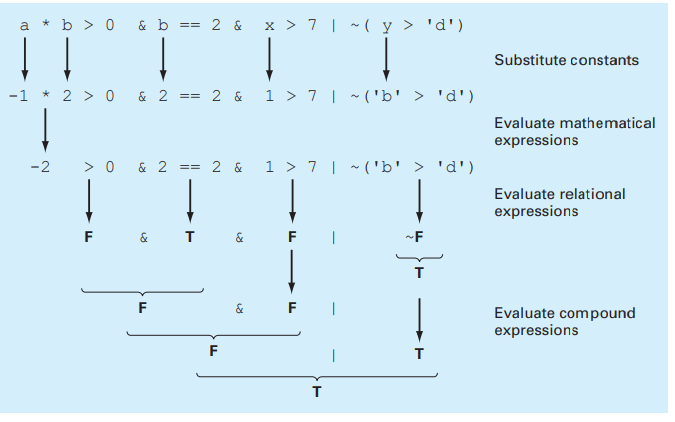
\includegraphics[width=0.8\linewidth]{fig_3_1}
    \caption{A step-by-step evaluation of a complex decision}
\end{figure}

\begin{lstlisting}[frame=none, numbers=none]
    elseif condition3
    statements3
    .
    .
    .
    else
    statementselse
    end
\end{lstlisting}

\section*{EXAMPLE 3.4 if Structures}

Problem Statement. For a scalar, the built-in MATLAB sign function returns the sign
of its argument (−1, 0, 1). Here’s a MATLAB session that illustrates how it works:

\begin{lstlisting}[frame=none, numbers=none]
    >> sign(25.6)
    ans =
         1
    >> sign(-0.776)
    ans =
        -1
    >> sign(0)
    ans =
        0
\end{lstlisting}
Develop an M-file to perform the same function.

Solution. First, an if structure can be used to return 1 if the argument is positive:
\begin{lstlisting}[frame=none, numbers=none]
    % mysign(x) returns 1 if x is greater than zero.
    if x > 0
    sgn = 1;
    end
\end{lstlisting}function sgn = mysign(x)

This function can be run as
\begin{lstlisting}[frame=none, numbers=none]
    >> mysign(25.6)
    ans =
          1
\end{lstlisting}
Although the function handles positive numbers correctly, if it is run with a negative
or zero argument, nothing is displayed. To partially remedy this shortcoming, an
if$\ldots$else structure can be used to display –1 if the condition is false:
function sgn = mysign(x)
\begin{lstlisting}[frame=none, numbers=none]
    % mysign(x) returns 1 if x is greater than zero.
    % -1 if x is less than or equal to zero.
    if x > 0
        sgn = 1;
    else
        sgn = -1;
    end
\end{lstlisting}
    This function can be run as

\begin{lstlisting}[frame=none, numbers=none]
    >> mysign(-0.776)
    ans =
         -1
\end{lstlisting}
Although the positive and negative cases are now handled properly, -1 is erroneously
returned if a zero argument is used. An if$\ldots$elseif structure can be used to incorporate
this final case:
function sgn = mysign(x)
\begin{lstlisting}[frame=none, numbers=none]
    % mysign(x) returns 1 if x is greater than zero.
    % -1 if x is less than zero.
    % 0 if x is equal to zero.
    if x > 0
        sgn = 1;
    elseif x < 0
        sgn = -1;
    else
        sgn = 0;
    end
\end{lstlisting}
    The function now handles all possible cases. For example,

\begin{lstlisting}[frame=none, numbers=none]
    >> mysign(0)
    ans =
         0
\end{lstlisting}

The switch Structure. The switch structure is similar in spirit to the \texttt{if$\ldots$elseif}
structure. However, rather than testing individual conditions, the branching is based on the
value of a single test expression. Depending on its value, different blocks of code are implemented. In addition, an optional block is implemented if the expression takes on none of
the prescribed values. It has the general syntax

\begin{lstlisting}[frame=none, numbers=none]
    switch testexpression
        case value1
    statements1
    case value2
        statements2
    .
    .
    .
    otherwise
        statements_otherwise
    end
\end{lstlisting}
As an example, here is function that displays a message depending on the value of the
string variable, \texttt{grade}.
\begin{lstlisting}[frame=none, numbers=none]
    grade = 'B';
    switch grade
        case 'A'
            disp('Excellent')
        case 'B'
            disp('Good')
        case 'C'
            disp('Mediocre')
        case 'D'
            disp('Whoops')
        case 'F'
            disp('Would like fries with your order?')
        otherwise
            disp('Huh!')
    end
\end{lstlisting}
When this code was executed, the message “Good” would be displayed.


Variable Argument List. MATLAB allows a variable number of arguments to be passed
to a function. This feature can come in handy for incorporating default values into your
functions. A default value is a number that is automatically assigned in the event that the
user does not pass it to a function.


As an example, recall that earlier in this chapter, we developed a function \texttt{freefall},
which had three arguments:
\begin{lstlisting}[frame=none, numbers=none]
    v = freefall(t,m,cd)
\end{lstlisting}
Although a user would obviously need to specify the time and mass, they might not have a
good idea of an appropriate drag coefficient. Therefore, it would be nice to have the 
program supply a value if they omitted it from the argument list.


MATLAB has a function called nargin that provides the number of input arguments
supplied to a function by a user. It can be used in conjunction with decision structures like

the if or switch constructs to incorporate default values as well as error messages into
your functions. The following code illustrates how this can be done for freefall:

\begin{lstlisting}[frame=none, numbers=none]
    function v = freefall2(t, m, cd)
    % freefall2: bungee velocity with second-order drag
    %   v=freefall2(t,m,cd) computes the free-fall velocity
    %               of an object with second-order drag.
    % input:
    %   t = time (s)
    %   m = mass (kg)
    %   cd = drag coefficient (default = 0.27 kg/m)
    % output:
    %   v = downward velocity (m/s)
    switch nargin
    case 0
        error('Must enter time and mass')
    case 1
        error('Must enter mass')
    case 2
        cd = 0.27;
    end
    g = 9.81; % acceleration of gravity
    v = sqrt(g * m / cd)*tanh(sqrt(g * cd / m) * t);
\end{lstlisting}
Notice how we have used a switch structure to either display error messages or set the
default, depending on the number of arguments passed by the user. Here is a command
window session showing the results:
\begin{lstlisting}[frame=none, numbers=none]
    >> freefall2(12,68.1,0.25)
    ans =
        50.6175
    >> freefall2(12,68.1)
    ans =
        48.8747
    >> freefall2(12)
    ??? Error using ==> freefall2 at 15
    Must enter mass
    >> freefall2()
    ??? Error using ==> freefall2 at 13
    Must enter time and mass
\end{lstlisting}

Note that nargin behaves a little differently when it is invoked in the command
window. In the command window, it must include a string argument specifying the function and it returns the number of arguments in the function. For example,
\begin{lstlisting}[frame=none, numbers=none]
    >> nargin('freefall2')
    ans =
            3
\end{lstlisting}


\subsection{Loops}


As the name implies, loops perform operations repetitively. There are two types of loops,
depending on how the repetitions are terminated. A for loop ends after a specified number
of repetitions. A while loop ends on the basis of a logical condition.
The for$\ldots$ end Structure. A for loop repeats statements a specific number of times. Its
general syntax is


\begin{lstlisting}[frame=none, numbers=none]
    >> b = [2;4;6;8;10]
\end{lstlisting}for index = start:step:finish
statements
end


The for loop operates as follows. The index is a variable that is set at an initial value,
start. The program then compares the index with a desired final value, finish. If the
index is less than or equal to the finish, the program executes the statements. When
it reaches the end line that marks the end of the loop, the index variable is increased by
the step and the program loops back up to the for statement. The process continues until
the index becomes greater than the finish value. At this point, the loop terminates as the
program skips down to the line immediately following the end statement.


Note that if an increment of 1 is desired (as is often the case), the step can be dropped.
For example,


\begin{lstlisting}[frame=none, numbers=none]
    >> b = [2;4;6;8;10]
\end{lstlisting}for i = 1:5
disp(i)
end
When this executes, MATLAB would display in succession, 1, 2, 3, 4, 5. In other
words, the default step is 1.


The size of the step can be changed from the default of 1 to any other numeric value.
It does not have to be an integer, nor does it have to be positive. For example, step sizes of
0.2, –1, or –5, are all acceptable.


If a negative step is used, the loop will “countdown” in reverse. For such cases, the
loop’s logic is reversed. Thus, the finish is less than the start and the loop terminates
when the index is less than the finish. For example,
\begin{lstlisting}[frame=none, numbers=none]
    >> b = [2;4;6;8;10]
\end{lstlisting}for j = 10:-1:1
disp(j)
end
When this executes, MATLAB would display the classic “countdown” sequence: 
\begin{lstlisting}[frame=none, numbers=none]
    >> b = [2;4;6;8;10]
\end{lstlisting}10, 9,
8, 7, 6, 5, 4, 3, 2, 1.


\section*{EXAMPLE 3.5 Using a for Loop to Compute the Factorial}

Problem Statement. Develop an M-file to compute the factorial.
\[\begin{array}{ll}
    0!& = 1\\
    1!& = 1\\
    2!& = 1 \times 2 = 2\\
    3!& = 1 \times 2 \times 3 = 6\\
    4!& = 1 \times 2 \times 3 \times 4 = 24\\
    5!& = 1 \times 2 \times 3 \times 4 \times 5 = 120\\ 
    \vdots \\
\end{array} \]


Solution. A simple function to implement this calculation can be developed as
function fout = factor(n)
\begin{lstlisting}[frame=none, numbers=none]
    % factor(n):
    % Computes the product of all the integers from 1 to n.
    x = 1;
    for i = 1:n
        x = x * i;
    end
    fout = x;
    end
\end{lstlisting}
which can be run as
\begin{lstlisting}[frame=none, numbers=none]
    >> factor(5)
    ans =
         120
\end{lstlisting}
This loop will execute 5 times (from 1 to 5). At the end of the process, x will hold a value
of 5! (meaning 5 factorial or 1 $\times$ 2 $\times$ 3 $\times$ 4 $\times$ 5 = 120).
Notice what happens if n = 0. For this case, the for loop would not execute, and we
would get the desired result, 0! = 1.


\noindent \textbf{Vectorization}. The \texttt{for} loop is easy to implement and understand. However, for MATLAB, it is not necessarily the most efficient means to repeat statements a specific number of times. Because of MATLAB's ability to operate directly on arrays, \emph{vectorization} provides a much more efficient option. For example, the following \texttt{for} loop structure:\\




\texttt{i=0;\\
\indent t=0: 0.02: 50\\
\indent\hspace{2mm} i=i+1;\\
\indent\hspace{2mm} y(i)=cos (t);\\
\indent end}\\

\noindent can be represented in vectorized form as\\

\texttt{t = 0:0.02:50;\\
\indent y = cos(t);\\}

\noindent It should be noted that for more complex code, it may not be obvious how to vectorize the code. That said, wherever possible, vectorization is recommended.
Preallocation of Memory. MATLAB automatically increases the size of arrays every time you add a new element. This can become time consuming when you perform actions such as adding new values one at a time within a loop. For example, here is some code that\\

\noindent\textbf{Preallocation of Memory.} MATLAB automatically increases the size of arrays every
time you add a new element. This can become time consuming when you perform actions
such as adding new values one at a time within a loop. For example, here is some code that
sets value of elements of \texttt{y} depending on whether or not values of t are greater than one:\\

\texttt{t = 0:.01:5;\\
\indent for i = 1:length(t)\\
\indent\hspace{2mm} if t(i)>1\\
\indent\hspace{4mm} y(i) = 1/t(i);\\
\indent\hspace{2mm} else\\
\indent\hspace{4mm} y(i) = 1;\\
\indent\hspace{2mm} end\\
\indent end\\}

\noindent For this case, MATLAB must resize \texttt{y} every time a new value is determined. The following
code preallocates the proper amount of memory by using a vectorized statement to
assign ones to y prior to entering the loop.\\

\texttt{t = 0:.01:5;\\
\indent y = ones(size(t));\\
\indent for i = 1:length(t)\\
\indent\hspace{2mm} if t(i)>1\\
\indent\hspace{4mm} y(i) = 1/t(i);\\
\indent\hspace{2mm} end\\
\indent end}\\

\noindent Thus, the array is only sized once. In addition, preallocation helps reduce memory fragmentation,
which also enhances efficiency.\\

\noindent\textbf{The \texttt{while} Structure.} A \texttt{while} loop repeats as long as a logical condition is true. Its
general syntax is\\

\texttt{while \emph{condition}\\
\indent\hspace{2mm} statements\\
\indent end}\\

\noindent The \emph{statements} between the \texttt{while} and the \texttt{end} are repeated as long as the \texttt{\emph{condition}} is
true. A simple example is\\

\texttt{x = 8\\
\indent while x > 0\\
\indent\hspace{2mm} x = x - 3\\
\indent\hspace{2mm} disp(x)\\
\indent end}\\

\noindent When this code is run, the result is\\

\texttt{x =\\
\indent\indent 8\\
\indent\indent 5\\
\indent\indent 2\\
\indent\indent -1}\\

\noindent\textbf{The \texttt{while...break} Structure.} Although the \texttt{while} structure is extremely useful, the
fact that it always exits at the beginning of the structure on a false result is somewhat
constraining. For this reason, languages such as Fortran 90 and Visual Basic have special
structures that allow loop termination on a true condition anywhere in the loop. Although
such structures are currently not available inMATLAB, their functionality can be mimicked
by a special version of the \texttt{while} loop. The syntax of this version, called a \texttt{while...break} structure, can be written as\\

\texttt{while (1)\\
\indent\hspace{2mm} \emph{statements}\\
\indent\hspace{2mm} if \emph{condition}, break, end\\
\indent\hspace{2mm} \emph{statements}\\
\indent end}\\

\noindent where \texttt{break} terminates execution of the loop. Thus, a single line \texttt{if} is used to exit the
loop if the condition tests true. Note that as shown, the \texttt{break} can be placed in the middle
of the loop (i.e., with statements before and after it). Such a structure is called a \emph{midtest}
\emph{loop}.\\
\indent If the problem required it, we could place the \texttt{break} at the very beginning to create a
\emph{pretest loop}. An example is\\

\texttt{while (1)\\
\indent\hspace{2mm} If x < 0, break, end\\
\indent\hspace{2mm} x = x - 5;\\
\indent end}\\

\noindent Notice how \texttt{5} is subtracted from \texttt{x} on each iteration. This represents a mechanism so that
the loop eventually terminates. Every decision loop must have such a mechanism. Otherwise
it would become a so-called \emph{infinite loop} that would never stop.\\
\indent Alternatively, we could also place the \texttt{if...break} statement at the very end and create
a \emph{posttest loop},\\

\texttt{while (1)\\
\indent\hspace{2mm} x = x - 5;\\
\indent\hspace{2mm} if x < 0, break, end\\
\indent end}\\

It should be clear that, in fact, all three structures are really the same. That is, depending
on where we put the exit (beginning, middle, or end) dictates whether we have a pre-,
mid- or posttest. It is this simplicity that led the computer scientists who developed
Fortran 90 and Visual Basic to favor this structure over other forms of the decision loop
such as the conventional \texttt{while} structure.\\

\noindent\textbf{The \texttt{pause} Command.} There are often times when you might want a program to temporarily
halt. The command \texttt{pause} causes a procedure to stop and wait until any key is hit.
A nice example involves creating a sequence of plots that a user might want to leisurely
peruse before moving on to the next. The following code employs a \texttt{for} loop to create a
sequence of interesting plots that can be viewed in this manner:\\

\texttt{for n = 3:10\\
\indent\hspace{2mm} mesh(magic(n))\\
\indent\hspace{2mm} pause\\
\indent end}\\

The \texttt{pause} can also be formulated as \texttt{pause(n)}, in which case the procedure will halt
for \texttt{n} seconds. This feature can be demonstrated by implementing it in conjunction with
several other useful MATLAB functions. The \texttt{beep} command causes the computer to emit
a beep sound. Two other functions, \texttt{tic} and \texttt{toc}, work together to measure elapsed time.
The \texttt{tic} command saves the current time that \texttt{toc} later employs to display the elapsed
time. The following code then confirms that \texttt{pause(n)} works as advertised complete with
sound effects:\\

\texttt{tic\\
\indent beep\\
\indent pause(5)\\
\indent beep\\
\indent toc}\\

\noindent When this code is run, the computer will beep. Five seconds later it will beep again and display
the following message:\\

\texttt{Elapsed time is 5.006306 seconds.}\\

\noindent By the way, if you ever have the urge to use the command \texttt{pause(inf)}, MATLAB will go
into an infinite loop. In such cases, you can return to the command prompt by typing
\textbf{Ctrl+c or Ctrl+Break}.
Although the foregoing examples might seem a tad frivolous, the commands can be
quite useful. For instance, \texttt{tic} and \texttt{toc} can be employed to identify the parts of an algorithm
that consume the most execution time. Further, the \textbf{Ctrl+c} or \textbf{Ctrl+Break} key combinations
come in real handy in the event that you inadvertently create an infinite loop in
one of your M-files.\\

\subsection{Animation}

\noindent There are two simple ways to animate a plot in MATLAB. First, if the computations are
sufficiently quick, the standard \texttt{plot} function can be employed in a way that the animation
can appear smooth. Here is a code fragment that indicates how a \texttt{for} loop and standard
plotting functions can be employed to animate a plot,\\

\texttt{\% create animation with standard plot functions\\
\indent for j=1:n\\
\indent \emph{plot commands}\\
\indent end}\\

\noindent Thus, because we do not include \texttt{hold on}, the plot will refresh on each loop iteration.
Through judicious use of axis commands, this can result in a smoothly changing image.\\
\indent Second, there are special functions, \texttt{getframe} and \texttt{movie}, that allow you to capture a
sequence of plots and then play them back. As the name implies, the \texttt{getframe} function
captures a snapshot (\emph{pixmap}) of the current axes or figure. It is usually used in a \texttt{for} loop
to assemble an array of movie frames for later playback with the \texttt{movie} function, which
has the following syntax:\\

\texttt{movie(m,n,fps)}\\

\noindent where \emph{m} = the vector or matrix holding the sequence of frames constituting the movie,
\emph{n} = an optional variable specifying how many times the movie is to be repeated (if it is
omitted, the movie plays once), and \emph{fps} = an optional variable that specifies the
movie's \emph{frame rate} (if it is omitted, the default is 12 frames per second). Here is a code
fragment that indicates how a \texttt{for} loop along with the two functions can be employed
to create a movie,\\

\texttt{\% create animation with standard plot functions\\
\indent for j=1:n\\
\indent\hspace{2mm} plot commands\\
\indent\hspace{2mm} M(j) = getframe;\\
\indent end\\
\indent movie(M)}\\

Each time the loop executes, the \texttt{\emph{plot commands}} create an updated version of a plot,
which is then stored in the vector M. After the loop terminates, the \texttt{n} images are then played
back by \texttt{movie}.\\

\begin{example} Animation of Projectile Motion
    \bigskip\\
    \textbf{Problem Statement.}\quad In the absence of air resistance, the Cartesian coordinates of a projectile
    launched with an initial velocity ($v_0$) and angle ($\theta_0$) can be computed with\\
    
    $x = v_0 \cos(\theta_0)t$\\
    \indent
    $y = v_0 \sin(\theta_0)t - 0.5gt^2$\\

    \noindent where $g = 9.81$ $m/s^2$. Develop a script to generate an animated plot of the projectile's
    trajectory given that $v_0 = 5$ m/s and $\theta_0 = 45^{\circ}$.\\

    \noindent\textbf{Solution}\quad A script to generate the animation can be written as\\

    \texttt{clc,clf,clear\\
    \indent g=9.81; theta0=45*pi/180; v0=5;\\
    \indent t(1)=0;x=0;y=0;\\
    \indent plot(x,y,'o','MarkerFaceColor','b','MarkerSize',8)\\
    \indent axis([0 3 0 0.8])\\
    \indent M(1)=getframe;\\
    \indent dt=1/128;\\
    \indent for j = 2:1000\\
    \indent\hspace{2mm} t(j)=t(j-1)+dt;\\
    \indent\hspace{2mm} x=v0*cos(theta0)*t(j);\\
    \indent\hspace{2mm} y=v0*sin(theta0)*t(j)-0.5*g*t(j)\textasciicircum2;\\
    \indent\hspace{2mm} plot(x,y,'o','MarkerFaceColor','b','MarkerSize',8)\\
    \indent\hspace{2mm} axis([0 3 0 0.8])\\
    \indent\hspace{2mm} M(j)=getframe;\\
    \indent\hspace{2mm} if y<=0, break, end\\
    \indent end\\
    \indent pause\\
    \indent movie(M, 1)}\\

    Several features of this script bear mention. First, notice that we have fixed the ranges for
the \emph{x} and \emph{y} axes. If this is not done, the axes will rescale and cause the animation to jump
around. Second, we terminate the \texttt{for} loop when the projectile's height y falls below zero.\\
\indent When the script is executed, two animations will be displayed (we've placed a \texttt{pause}
between them). The first corresponds to the sequential generation of the frames within the
loop, and the second corresponds to the actual movie. Although we cannot show the results
here, the trajectory for both cases will look like Fig. 3.2. You should enter and run the foregoing
script in MATLAB to see the actual animation.\\

\begin{figure}[h]
    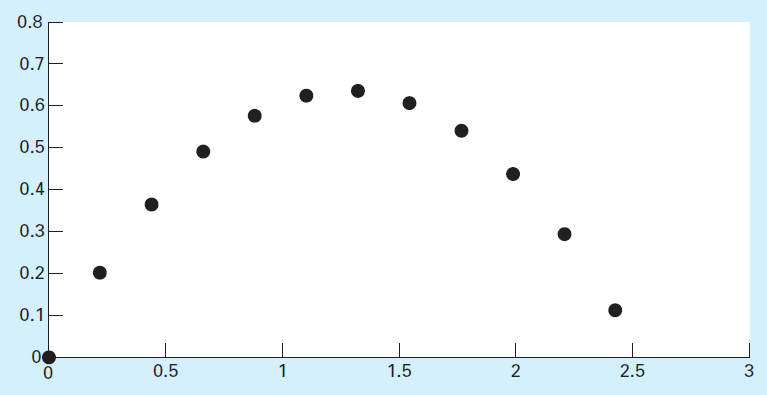
\includegraphics[width=0.70\linewidth]{./images/example_3_3_2}
    \caption{Plot of a projectile's trajectory.}
\end{figure}

\end{example}

\section{NESTING AND INDENTATION}
\noindent We need to understand that structures can be "nested" within each other. \emph{Nesting} refers to
placing structures within other structures. The following example illustrates the concept.\\

\begin{example} Nesting Structures\\
    \noindent\textbf{Problem Statement.}\quad The roots of a quadratic equation\\

    $f(x) = ax^2 + bx + c$\\

    \noindent can be determined with the quadratic formula\\

    $x = \dfrac{-b +- \sqrt{b^2 - 4ac}}{2a}$\\

    \noindent\textbf{Solution}\quad \emph{Top-down design} provides a nice approach for designing an algorithm to compute
    the roots. This involves developing the general structure without details and then
    refining the algorithm. To start, we first recognize that depending on whether the parameter
    \emph{a} is zero, we will either have "special" cases (e.g., single roots or trivial values) or conventional
    cases using the quadratic formula. This "big-picture" version can be programmed as\\

    \texttt{function quadroots(a, b, c)\\
    \indent \% quadroots: roots of quadratic equation\\
    \indent \% \hspace{2mm} quadroots(a,b,c): real and complex roots\\
    \indent \% \indent\indent of quadratic equation\\
    \indent \% input:\\
    \indent \% \hspace{2mm} a = second-order coefficient\\
    \indent \% \hspace{2mm} b = first-order coefficient\\
    \indent \% \hspace{2mm} c = zero-order coefficient\\
    \indent \% output:\\
    \indent \% \hspace{2mm} r1 = real part of first root\\
    \indent \% \hspace{2mm} i1 = imaginary part of first root\\
    \indent \% \hspace{2mm} r2 = real part of second root\\
    \indent \% \hspace{2mm} i2 = imaginary part of second root\\
    \indent if a == 0\\
    \indent\hspace{2mm} \%special cases\\
    \indent else\\
    \indent\hspace{2mm} \%quadratic formula\\
    \indent end
    }\\

    \noindent Next, we develop refined code to handle the "special" cases:\\

    \texttt{\%special cases\\
    \indent if b $\sim$= 0\\
    \indent\hspace{2mm} \%single root\\
    \indent\hspace{2mm} r1 = -c / b\\
    \indent else\\
    \indent\hspace{2mm} \%trivial solution\\
    \indent\hspace{2mm} disp('Trivial solution. Try again')\\
    \indent end}\\
    
    \noindent And we can develop refined code to handle the quadratic formula cases:\\

    \texttt{\%quadratic formula\\
    \indent d = b \textasciicircum2 - 4 * a * c;\\
    \indent if d >= 0\\
    \indent\hspace{2mm} \%real roots\\
    \indent\hspace{2mm} r1 = (-b + sqrt(d)) / (2 * a)\\
    \indent\hspace{2mm} r2 = (-b - sqrt(d)) / (2 * a)\\
    \indent else\\
    \indent\hspace{2mm} \%complex roots\\
    \indent\hspace{2mm} r1 = -b / (2 * a)\\
    \indent\hspace{2mm} i1 = sqrt(abs(d)) / (2 * a)\\
    \indent\hspace{2mm} r2 = r1\\
    \indent\hspace{2mm} i2 = -i1\\
    \indent end}\\

    We can then merely substitute these blocks back into the simple "big-picture" framework
to give the final result:

    \texttt{function quadroots(a, b, c)\\
    \indent \% quadroots: roots of quadratic equation\\
    \indent \% \hspace{2mm}quadroots(a,b,c): real and complex roots\\
    \indent \% \indent\indent of quadratic equation\\
    \indent \% input:\\
    \indent \% \hspace{2mm}a = second-order coefficient\\
    \indent \% \hspace{2mm}b = first-order coefficient\\
    \indent \% \hspace{2mm}c = zero-order coefficient\\
    \indent \% output:\\
    \indent \% \hspace{2mm}r1 = real part of first root\\
    \indent \% \hspace{2mm}i1 = imaginary part of first root\\
    \indent \% \hspace{2mm}r2 = real part of second root\\
    \indent \% \hspace{2mm}i2 = imaginary part of second root\\
    \indent if a == 0}\\

    \begin{figure}[h]
        \begin{lstlisting}[numbers=none]
            %special cases
            if b ~= 0
            %single root
            r1 = -c / b
            else
            %trivial solution
            disp('Trivial solution. Try again')
            end
        \end{lstlisting}
    \end{figure}

    \texttt{else}\\

    \begin{figure}[h]
        \begin{lstlisting}[numbers=none]
            %quadratic formula
            d = b ^ 2 - 4 * a * c; %discriminant
            if d >= 0
            %real roots
            r1 = (-b + sqrt(d)) / (2 * a)
            r2 = (-b - sqrt(d)) / (2 * a)
            else
            %complex roots
            r1 = -b / (2 * a)
            i1 = sqrt(abs(d)) / (2 * a)
            r2 = r1
            i2 = -i1
            end
        \end{lstlisting}
    \end{figure}

    \texttt{end}\\

    As highlighted by the shading, notice how indentation helps to make the underlying
logical structure clear. Also notice how "modular" the structures are. Here is a command
window session illustrating how the function performs:\\

\texttt{>> quadroots(1,1,1)\\
\indent r1 =\\
\indent \hspace{2mm}-0.5000\\
\indent i1 =\\
\indent \hspace{2mm}0.8660\\
\indent r2 =\\
\indent \hspace{2mm}-0.5000\\
\indent i2 =\\
\indent \hspace{2mm}-0.8660\\
\indent >> quadroots(1,5,1)\\
\indent r1 =\\
\indent \hspace{2mm}-0.2087\\
\indent r2 =\\
\indent \hspace{2mm}-4.7913\\
\indent >> quadroots(0,5,1)\\
\indent r1 =\\
\indent \hspace{2mm}-0.2000\\
\indent >> quadroots(0, 0, 0)\\
\indent Trivial solution. Try again}\\

\end{example}

\section{PASSING FUNCTIONS TO M-FILES}
\noindent
Much of the remainder of the book involves developing functions to numerically evaluate
other functions. Although a customized function could be developed for every new equation
we analyzed, a better alternative is to design a generic function and pass the particular
equation we wish to analyze as an argument. In the parlance of MATLAB, these functions
are given a special name: \emph{function functions}. Before describing how they work, we will
first introduce anonymous functions, which provide a handy means to define simple userdefined
functions without developing a full-blown M-file.\\

\subsection{Anonymous Functions}
\noindent
\emph{Anonymous functions} allow you to create a simple function without creating an M-file.
They can be defined within the command window with the following syntax:\\

\texttt{fhandle = @(arglist) \emph{expression}}\\

\noindent
where \texttt{fhandle} = the function handle you can use to invoke the function, \texttt{arglist} = a
comma separated list of input arguments to be passed to the function, and \texttt{expression} =
any single valid MATLAB expression. For example,\\

\texttt{>> f1=@(x,y) x\textasciicircum2 + y\textasciicircum2;}\\

\noindent
Once these functions are defined in the command window, they can be used just as other
functions:\\

\texttt{>> f1(3,4)\\
\indent ans =\\
\indent\hspace{2mm} 25}\\

Aside from the variables in its argument list, an anonymous function can include variables
that exist in the workspace where it is created. For example, we could create an
anonymous function $f(x) = 4x^2$ as\\

\texttt{>> a = 4;\\
\indent >> b = 2;\\
\indent >> f2=@(x) a*x\textasciicircum b;\\
\indent >> f2(3)\\
\indent ans = 36}\\

Note that if subsequently we enter new values for \texttt{a} and \texttt{b}, the anonymous function
does not change:\\

\texttt{>> a = 3;\\
\indent >> f2(3)\\
\indent ans = 36}\\

\noindent
Thus, the function handle holds a snapshot of the function at the time it was created. If we
want the variables to take on values, we must recreate the function. For example, having
changed \texttt{a} to 3,\\

\texttt{>> f2=@(x) a*x\textasciicircum b;}\\

\noindent with the result\\

\texttt{>> f2(3)\\
\indent ans =\\ 
\indent\hspace{2mm} 27}\\

It should be noted that prior to MATLAB 7, \texttt{inline} functions performed the same
role as anonymous functions. For example, the anonymous function developed above, \texttt{f1},
could be written as\\

\texttt{>> f1=inline('x\textasciicircum 2 + y\textasciicircum 2','x','y');}\\

\noindent
Although they are being phased out in favor of anonymous function, some readers might be
using earlier versions, and so we thought it would be helpful to mention them. MATLAB
help can be consulted to learn more about their use and limitations.

\subsection{Function Functions}
\noindent
\emph{Function functions} are functions that operate on other functions which are passed to it as
input arguments. The function that is passed to the function function is referred to as the
\emph{passed function}. A simple example is the built-in function \texttt{fplot}, which plots the graphs
of functions. A simple representation of its syntax is\\

\texttt{fplot(func,lims)}\\

where \texttt{func} is the function being plotted between the \emph{x}-axis limits specified by \texttt{lims = [xmin xmax]}. 
For this case, \texttt{func} is the passed function. This function is "smart" in that it
automatically analyzes the function and decides how many values to use so that the plot
will exhibit all the function's features.\\
\indent Here is an example of how \texttt{fplot} can be used to plot the velocity of the free-falling
bungee jumper. The function can be created with an anonymous function:\\

\texttt{>> vel=@(t) ...\\
\indent sqrt(9.81*68.1/0.25)*tanh(sqrt(9.81*0.25/68.1)*t);}\\

\noindent We can then generate a plot from $t$ = 0 to 12 as\\

\texttt{>> fplot(vel,[0 12])}\\

\noindent The result is displayed in Fig. 3.3.\\
\indent Note that in the remainder of this book, we will have many occasions to use MATLAB's
built-in function functions. As in the following example, we will also be developing
our own.\\

\begin{figure}[h]
    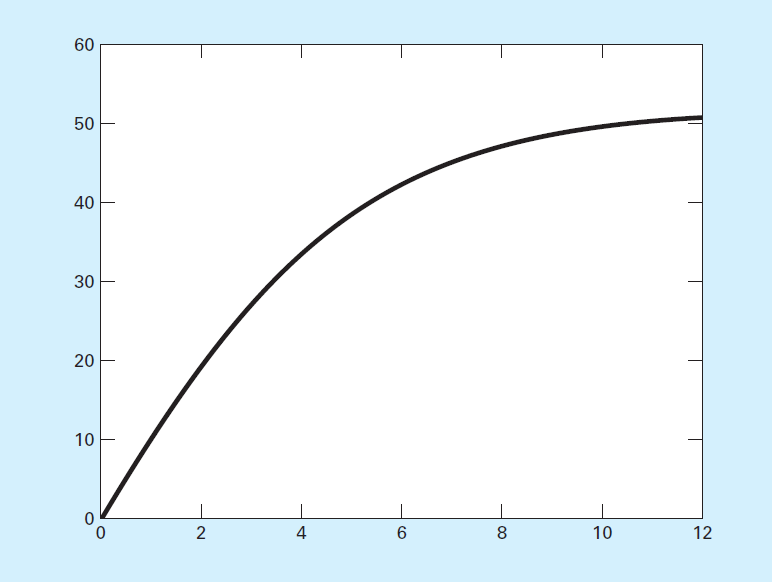
\includegraphics[width=0.5\linewidth]{./images/fig_3_3}
    \caption{A plot of velocity versus time generated with the \texttt{fplot} function.}
\end{figure}

\begin{example} Building and Implementing a Function Function
    \noindent\textbf{Problem Statement.}\quad Develop an M-file function function to determine the average value
    of a function over a range. Illustrate its use for the bungee jumper velocity over the range
    from $t$ = 0 to 12 s:\\

    $v(t) = \sqrt{\dfrac{gm}{c_d}}tanh\Big(\sqrt{\dfrac{gc_d}{m}}t \Big)$\\

    \noindent where $g = 9.81$, $m = 68.1$, and $c_d = 0.25$.\\

    \noindent\textbf{Solution.}\quad The average value of the function can be computed with standard MATLAB
    commands as\\

    \texttt{>> t=linspace(0,12);\\
    \indent >> v=sqrt(9.81*68.1/0.25)*tanh(sqrt(9.81*0.25/68.1)*t);\\
    \indent >> mean(v)\\
    \indent ans =\\
    \indent\hspace{2mm} 36.0870}\\

    \noindent
    Inspection of a plot of the function (Fig. 3.3) shows that this result is a reasonable estimate
    of the curve's average height.\\

    We can write an M-file to perform the same computation:\\

    \texttt{function favg = funcavg(a,b,n)\\
    \indent \% funcavg: average function height\\
    \indent \% \hspace{2mm}favg=funcavg(a,b,n): computes average value\\
    \indent \% \indent\indent of function over a range\\
    \indent \% input:\\
    \indent \% \hspace{2mm}a = lower bound of range\\
    \indent \% \hspace{2mm}b = upper bound of range\\
    \indent \% \hspace{2mm}n = number of intervals\\
    \indent \% output:\\
    \indent \% \hspace{2mm}favg = average value of function\\
    \indent x = linspace(a,b,n);\\
    \indent y = func(x);\\
    \indent favg = mean(y);\\
    \indent end\\
    \indent function f = func(t)\\
    \indent f=sqrt(9.81*68.1/0.25)*tanh(sqrt(9.81*0.25/68.1)*t);\\
    \indent end}\\

    The main function first uses \texttt{linspace} to generate equally spaced $x$ values across
    the range. These values are then passed to a subfunction \texttt{func} in order to generate the corresponding
    y values. Finally, the average value is computed. The function can be run from
    the command window as\\

    \texttt{>> funcavg (0,12,60)\\
    \indent ans =\\
    \indent\hspace{2mm} 36.0127}\\

    Now let's rewrite the M-file so that rather than being specific to \texttt{func}, it evaluates a
    nonspecific function name f that is passed in as an argument:\\

    \texttt{function favg = funcavg (f,a,b,n)\\
    \indent \% funcavg: average function height\\
    \indent \% \hspace{2mm}favg=funcavg(f,a,b,n): computes average value\\
    \indent \% \indent\indent of function over a range\\
    \indent \% input:\\
    \indent \% \hspace{2mm}f = function to be evaluated\\
    \indent \% \hspace{2mm}a = lower bound of range\\
    \indent \% \hspace{2mm}b = upper bound of range\\
    \indent \% \hspace{2mm}n = number of intervals\\
    \indent \% output:\\
    \indent \% \hspace{2mm}favg = average value of function\\
    \indent x = linspace(a,b,n);\\
    \indent y = f(x);\\
    \indent favg = mean(y);}\\

    \noindent Because we have removed the subfunction \texttt{func}, this version is truly generic. It can be run
    from the command window as\\

    \texttt{>> vel=@(t) ...\\
    \indent sqrt(9.81*68.1/0.25)*tanh(sqrt(9.81*0.25/68.1)*t);\\
    \indent >> funcavg(vel,0,12,60)\\
    \indent ans =\\
    \indent\hspace{2mm} 36.0127}\\

    To demonstrate its generic nature, \texttt{funcavg} can easily be applied to another case by
merely passing it a different function. For example, it could be used to determine the average
value of the built-in \texttt{sin} function between 0 and $2\pi$ as\\

    \texttt{>> funcavg(@sin,0,2*pi,180)\\
    \indent ans =\\
    \indent\hspace{2mm} -6.3001e-017}\\

    Does this result make sense?\\
    \indent We can see that \texttt{funcavg} is now designed to evaluate any valid MATLAB expression.
    We will do this on numerous occasions throughout the remainder of this text in a
    number of contexts ranging from nonlinear equation solving to the solution of differential
    equations.\\

\end{example}

\subsection{Passing Parameters}
\noindent
Recall from Chap. 1 that the terms in mathematical models can be divided into dependent
and independent variables, parameters, and forcing functions. For the bungee jumper
model, the velocity ($v$) is the dependent variable, time ($t$) is the independent variable, the
mass ($m$) and drag coefficient ($c_d$) are parameters, and the gravitational constant ($g$) is the
forcing function. It is commonplace to investigate the behavior of such models by performing
a \emph{sensitivity analysis}. This involves observing how the dependent variable changes
as the parameters and forcing functions are varied.\\
\indent In Example 3.8, we developed a function function, \texttt{funcavg}, and used it to determine
the average value of the bungee jumper velocity for the case where the parameters were set
at $m = 68.1$ and $c_d= 0.25$. Suppose that we wanted to analyze the same function, but with
different parameters. Of course, we could retype the function with new values for each
case, but it would be preferable to just change the parameters.\\
\indent As we learned in Sec. 3.5.1, it is possible to incorporate parameters into anonymous
functions. For example, rather than "wiring" the numeric values, we could have done the
following:\\

\texttt{>> m=68.1;cd=0.25;\\
\indent >> vel=@(t) sqrt(9.81*m/cd)*tanh(sqrt(9.81*cd/m)*t);\\
\indent >> funcavg(vel,0,12,60)\\
\indent ans =\\
\indent\hspace{2mm} 36.0127}\\

\noindent However, if we want the parameters to take on new values, we must recreate the anonymous
function.\\
\indent MATLAB offers a better alternative by adding the term \texttt{varargin} as the function
function's last input argument. In addition, every time the passed function is invoked
within the function function, the term \texttt{varargin\{:\}} should be added to the end of its
argument list (note the curly brackets). Here is how both modifications can be implemented
for \texttt{funcavg} (omitting comments for conciseness):\\

\texttt{function favg = funcavg(f,a,b,n,varargin)\\
\indent x = linspace(a,b,n);\\
\indent y = f(x,varargin{:});\\
\indent favg = mean(y);}\\

When the passed function is defined, the actual parameters should be added at the end
of the argument list. If we used an anonymous function, this can be done as in\\

\texttt{>> vel=@(t,m,cd) sqrt(9.81*m/cd)*tanh(sqrt(9.81*cd/m)*t);}\\

\noindent
When all these changes have been made, analyzing different parameters becomes easy. To
implement the case where $m = 68.1$ and $c_d = 0.25$, we could enter\\

\texttt{>> funcavg(vel,0,12,60,68.1,0.25)\\
\indent ans =\\
\indent\hspace{2mm} 36.0127}\\

\noindent
An alternative case, say $m = 100$ and $c_d = 0.28$, could be rapidly generated by merely
changing the arguments:\\

\texttt{>> funcavg(vel,0,12,60,100,0.28)\\
\indent ans =\\
\indent\hspace{2mm} 38.9345}\\

\section{CASE STUDY - BUNGEE JUMPER VELOCITY}
\noindent\textbf{Background.}\quad In this section, we will use MATLAB to solve the free-falling bungee
jumper problem we posed at the beginning of this chapter. This involves obtaining a solution
of\\

$\dfrac{dv}{dt} = g - \dfrac{c_d}{m}v\left\lvert v \right\rvert$\\

Recall that, given an initial condition for time and velocity, the problem involved iteratively
solving the formula,\\

$v_{i+1} = v_i + \dfrac{dv_i}{dt}\Delta t$\\

\noindent Now also remember that to attain good accuracy, we would employ small steps. Therefore,
we would probably want to apply the formula repeatedly to step out from our initial time
to attain the value at the final time. Consequently, an algorithm to solve the problem would
be based on a loop.\\

\noindent\textbf{Solution.} Suppose that we started the computation at $t = 0$ and wanted to predict
velocity at $t = 12$ s using a time step of $\Delta t = 0.5$ s. We would therefore need to apply the
iterative equation 24 times---that is,\\

$n = \dfrac{12}{0.5} = 24$\\

\noindent
where n = the number of iterations of the loop. Because this result is exact (i.e., the ratio is
an integer), we can use a \texttt{for} loop as the basis for the algorithm. Here's an M-file to do this
including a subfunction defining the differential equation:\\

\texttt{function vend = velocity1(dt, ti, tf, vi)\\
\indent \% velocity1: Euler solution for bungee velocity\\
\indent \% \hspace{2mm}vend = velocity1(dt, ti, tf, vi)\\
\indent \% \indent\indent Euler method solution of bungee\\
\indent \% \indent\indent jumper velocity\\
\indent \% input:\\
\indent \% \hspace{2mm}dt = time step (s)\\
\indent \% \hspace{2mm}ti = initial time (s)\\
\indent \% \hspace{2mm}tf = final time (s)\\
\indent \% \hspace{2mm}vi = initial value of dependent variable (m/s)\\
\indent \% output:\\
\indent \% \hspace{2mm}vend = velocity at tf (m/s)\\
\indent t = ti;\\
\indent v = vi;\\
\indent n = (tf - ti) / dt;\\
\indent for i = 1:n\\
\indent \hspace{2mm}dvdt = deriv(v);\\
\indent \hspace{2mm}v = v + dvdt * dt;\\
\indent \hspace{2mm}t = t + dt;\\
\indent end\\
\indent vend = v;\\
\indent end\\
\indent function dv = deriv(v)\\
\indent dv = 9.81 - (0.25 / 68.1) * v*abs(v);\\
\indent end}\\

\noindent This function can be invoked from the command window with the result:\\

\texttt{>> velocity1(0.5,0,12,0)\\
\indent ans =\\
\indent\hspace{2mm} 50.9259}\\

Note that the true value obtained from the analytical solution is 50.6175 (Example
3.1). We can then try a much smaller value of \texttt{dt} to obtain a more accurate numerical
result:\\

\texttt{>> velocity1(0.001,0,12,0)\\
\indent ans =\\
\indent\hspace{2mm} 50.6181}\\

Although this function is certainly simple to program, it is not foolproof. In particular,
it will not work if the computation interval is not evenly divisible by the time step.
To cover such cases, a \texttt{while...break} loop can be substituted in place of the
shaded area (note that we have omitted the comments for conciseness):\\

\texttt{function vend = velocity2(dt, ti, tf, vi)\\
\indent t = ti;\\
\indent v = vi;\\
\indent h = dt;\\
\indent while(1)
\indent \hspace{2mm}if t + dt > tf, h = tf - t; end\\
\indent \hspace{2mm}dvdt = deriv(v);\\
\indent \hspace{2mm}v = v + dvdt * h;\\
\indent \hspace{2mm}t = t + h;\\
\indent \hspace{2mm}if t >= tf, break, end\\
\indent end\\
\indent vend = v;\\
\indent end\\
\indent function dv = deriv(v)\\
\indent dv = 9.81 - (0.25 / 68.1) * v*abs(v);\\
\indent end}\\

As soon as we enter the \texttt{while} loop, we use a single line \texttt{if} structure to test whether
adding \texttt{t + dt} will take us beyond the end of the interval. If not (which would usually be
the case at first), we do nothing. If so, we would shorten up the interval---that is, we set the
variable step h to the interval remaining: \texttt{tf - t}. By doing this, we guarantee that the last
step falls exactly on \texttt{tf}. After we implement this final step, the loop will terminate because
the condition \texttt{t >= tf} will test true.\\
\indent Notice that before entering the loop, we assign the value of the time step dt to another
variable \texttt{h}. We create this \emph{dummy variable} so that our routine does not change the given
value of dt if and when we shorten the time step. We do this in anticipation that we might
need to use the original value of dt somewhere else in the event that this code were integrated
within a larger program.\\
\indent If we run this new version, the result will be the same as for the version based on the
\texttt{for} loop structure:\\

\texttt{>> velocity2(0.5,0,12,0)\\
\indent ans =\\
\indent\hspace{2mm} 50.9259}\\

\noindent Further, we can use a dt that is not evenly divisible into \texttt{tf - ti}:\\

\texttt{>> velocity2(0.35,0,12,0)\\
\indent ans =\\
\indent\hspace{2mm} 50.8348}\\

We should note that the algorithm is still not foolproof. For example, the user could
have mistakenly entered a step size greater than the calculation interval (e.g., \texttt{tf - ti = 5}
and \texttt{dt = 20}). Thus, you might want to include error traps in your code to catch such errors
and then allow the user to correct the mistake.\\

As a final note, we should recognize that the foregoing code is not generic. That is, we
have designed it to solve the specific problem of the velocity of the bungee jumper. Amore
generic version can be developed as\\

\texttt{function yend = odesimp(dydt, dt, ti, tf, yi)\\
\indent t = ti; y = yi; h = dt;\\
\indent while (1)\\
\indent \hspace{2mm}if t + dt > tf, h = tf - t; end\\
\indent \hspace{2mm}y = y + dydt(y) * h;\\
\indent \hspace{2mm}t = t + h;\\
\indent \hspace{2mm}if t >= tf, break, end\\
\indent end\\
\indent yend = y;}\\

Notice how we have stripped out the parts of the algorithm that were specific to
the bungee example (including the subfunction defining the differential equation)
while keeping the essential features of the solution technique. We can then use this
routine to solve the bungee jumper example, by specifying the differential equation
with an anonymous function and passing its function handle to \texttt{odesimp} to generate
the solution\\

\texttt{>> dvdt=@(v) 9.81-(0.25/68.1)*v*abs(v);\\
\indent >> odesimp(dvdt,0.5,0,12,0)\\
\indent ans =\\
\indent\hspace{2mm}50.9259}\\

We could then analyze a different function without having to go in and modify the
M-file. For example, if y = 10 at t = 0, the differential equation $dy/dt=-0.1y$ has the analytical
solution $y = 10e^{-0.1t}$. Therefore, the solution at t = 5 would be $y(5) = 10^{e-0.1(5)} = 6.0653$.
We can use \texttt{odesimp} to obtain the same result numerically as in\\

\texttt{>> odesimp(@(y) -0.1*y,0.005,0,5,10)\\
\indent ans =\\
\indent\hspace{2mm} 6.0645}\\
\bigskip

\noindent\textbf{PROBLEMS}\\

\begin{multicols}{2}
    \noindent\textbf{3.1} Figure P3.1 shows a cylindrical tank with a conical
    base. If the liquid level is quite low, in the conical part, the
    volume is simply the conical volume of liquid. If the liquid
    level is midrange in the cylindrical part, the total volume of
    liquid includes the filled conical part and the partially filled
    cylindrical part.\\
    \indent Use decisional structures to write an M-file to compute
    the tank's volume as a function of given values of R and d.
    Design the function so that it returns the volume for all cases\\

    \noindent
    \begin{minipage}{\linewidth}
        \centering
        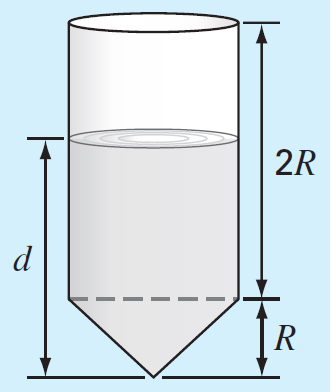
\includegraphics[width=0.4\linewidth]{./images/problem_3_3_1}
        \captionof*{figure}{Figure P3.1}
    \end{minipage}

    \noindent
    where the depth is less than $3R$. Return an error message
    ("Overtop") if you overtop the tank---that is, $d > 3R$. Test it
    with the following data:\\

    \noindent
    \begin{minipage}{\linewidth}
        \centering
        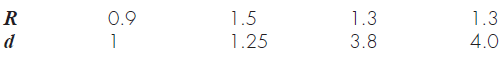
\includegraphics[width=0.9\linewidth]{./images/problem_3_3_2}
    \end{minipage}

    \noindent Note that the tank's radius is \textbf{R}.\\

    \noindent\textbf{3.2} An amount of money \emph{P} is invested in an account where
    interest is compounded at the end of the period. The future
    worth \emph{F} yielded at an interest rate \emph{i} after \emph{n} periods may be
    determined from the following formula:\\

    $F = P(1+i)^n$\\

    \noindent
    Write an M-file that will calculate the future worth of an investment
    for each year from 1 through $n$. The input to the
    function should include the initial investment $P$, the interest
    rate $i$ (as a decimal), and the number of years $n$ for which the
    future worth is to be calculated. The output should consist of
    a table with headings and columns for $n$ and $F$. Run the program
    for $P = \$100,000$, $i = 0.05$, and $n = 10$ years.\\

    \noindent\textbf{3.3} Economic formulas are available to compute annual
    payments for loans. Suppose that you borrow an amount of
    money $P$ and agree to repay it in $n$ annual payments at an
    interest rate of $i$. The formula to compute the annual payment
    $A$ is\\

    $A = P\dfrac{i(1+i)^n}{(1+i)^n - 1}$\\

    \noindent
    Write an M-file to compute A. Test it with $P$ = \$100,000 and
    an interest rate of $3.3\%$ $(i = 0.033)$. Compute results for $n$ =
    1, 2, 3, 4, and 5 and display the results as a table with headings
    and columns for $n$ and $A$.\\

    \noindent\textbf{3.4} The average daily temperature for an area can be approximated
    by the following function:\\

    $T = T_{mean} + (T_{peak}-T_{mean})cos(\omega(t-t_{peak}))$\\

    \noindent where $T_{mean}$ = the average annual temperature, $T_{peak}$ = the
    peak temperature, $\omega$ = the frequency of the annual variation ($=2\pi/365$),
    and $t_{peak}$ = day of the peak temperature ($\cong 205 d$). Parameters for some
    U.S. towns are listed here:\\

    \noindent
    \begin{minipage}{\linewidth}
        \centering
        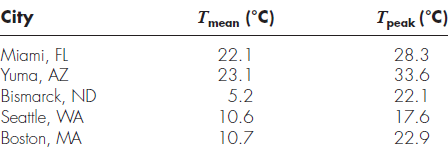
\includegraphics[width=0.9\linewidth]{./images/problem_3_3_3}
    \end{minipage}

    \noindent
    Develop an M-file that computes the average temperature
    between two days of the year for a particular city. Test it
    for (\textbf{a}) January--February in Yuma, AZ ($t$ = 0 to 59) and
    (\textbf{b}) July--August temperature in Seattle, WA($t$ = 180 to 242).\\

    \noindent\textbf{3.5} The sine function can be evaluated by the following
    infinite series:\\

    $sinx = x-\dfrac{x^3}{3!} + \dfrac{x^5}{5!} - \hdots$\\

    \noindent
    Create an M-file to implement this formula so that it computes
    and displays the values of $sin x$ as each term in the
    series is added. In other words, compute and display in
    sequence the values for\\

    $sinx = x$\\

    $sinx = x - \dfrac{x^3}{3!}$\\

    $sinx = x-\dfrac{x^3}{3!} + \dfrac{x^5}{5!}$\\

    \indent\indent$\vdots$\\

    \noindent
    up to the order term of your choosing. For each of the preceding,
    compute and display the percent relative error as\\

    $\%error = \dfrac{\text{true - series approximation}}{\text{true}}\times 100\%$\\

    \noindent
    As a test case, employ the program to compute $sin(0.9)$ for
    up to and including eight terms---that is, up to the term
    $x^{15}/15!$.\\

    \noindent\textbf{3.6} Two distances are required to specify the location of a
    point relative to an origin in two-dimensional space (Fig. P3.6):
    \begin{itemize}
        \item The horizontal and vertical distances $(x, y)$ in Cartesian
        coordinates.
        \item The radius and angle $(r, \theta)$ in polar coordinates.
    \end{itemize}

    \noindent
    It is relatively straightforward to compute Cartesian coordinates
    $(x, y)$ on the basis of polar coordinates $(r, \theta)$. The
    reverse process is not so simple. The radius can be computed
    by the following formula:\\

    $r = \sqrt{x^2 + y^2}$\\

    \noindent If the coordinates lie within the first and fourth coordinates
    (i.e., $x > 0$), then a simple formula can be used to
    compute $\theta$:\\

    $\theta = tan^{-1}\Big(\dfrac{y}{x} \Big)$\\

    \noindent
    \begin{minipage}{\linewidth}
        \centering
        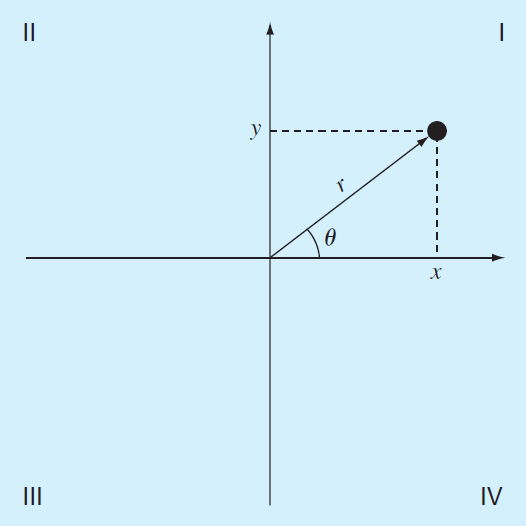
\includegraphics[width=0.9\linewidth]{./images/problem_3_3_4}
        \captionof*{figure}{Figure P3.6}
    \end{minipage}


    \noindent The difficulty arises for the other cases. The following table
    summarizes the possibilities:\\

    \noindent
    \begin{minipage}{\linewidth}
        \centering
        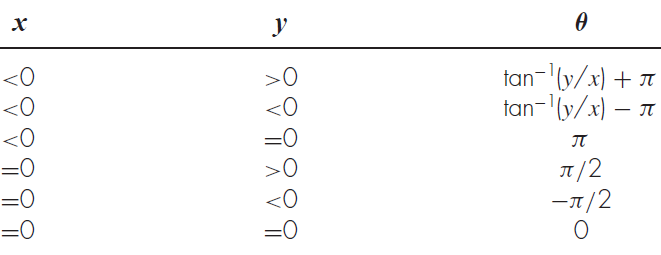
\includegraphics[width=0.9\linewidth]{./images/problem_3_3_5}
    \end{minipage}

    \noindent
    Write a well-structured M-file using \texttt{if...elseif} structures
    to calculate $r$ and $\theta$ as a function of $x$ and $y$. Express the
    final results for $\theta$ in degrees. Test your program by evaluating
    the following cases:\\

    \noindent
    \begin{minipage}{\linewidth}
        \centering
        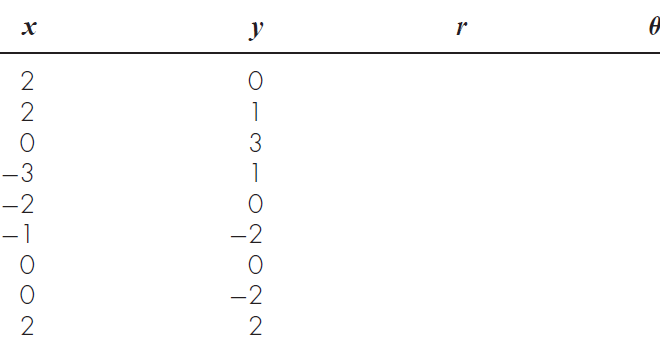
\includegraphics[width=0.9\linewidth]{./images/problem_3_3_6}
    \end{minipage}

    \noindent\textbf{3.7} Develop an M-file to determine polar coordinates as
    described in Prob. 3.6. However, rather than designing the
    function to evaluate a single case, pass vectors of $x$ and $y$.
    Have the function display the results as a table with columns
    for $x$, $y$, $r$, and $\theta$. Test the program for the cases outlined in
    Prob. 3.6.\\

    \noindent\textbf{3.8} Develop an M-file function that is passed a numeric
    grade from 0 to 100 and returns a letter grade according to
    the scheme:\\

    \noindent
    \begin{minipage}{\linewidth}
        \centering
        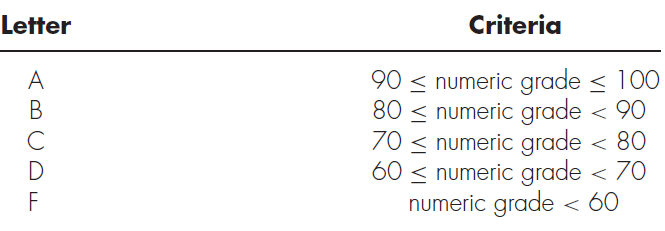
\includegraphics[width=0.9\linewidth]{./images/problem_3_3_7}
    \end{minipage}

    \noindent The first line of the function should be\\

    \texttt{function grade = lettergrade(score)}\\

    \noindent
    Design the function so that it displays an error message and
    terminates in the event that the user enters a value of \texttt{score}
    that is less than zero or greater than 100. Test your function
    with 89.9999, 90, 45 and 120.

    \noindent\textbf{3.9} Manning's equation can be used to compute the velocity
    of water in a rectangular open channel:\\

    $U = \dfrac{\sqrt{S}}{n}\Big(\dfrac{BH}{B + 2H} \Big)^{2/3}$\\

    \noindent where $U$ = velocity (m/s), $S$ = channel slope, $n$ = roughness
    coefficient, $B$ = width (m), and $H$ = depth (m). The following
    data are available for five channels:

    \noindent
    \begin{minipage}{\linewidth}
        \centering
        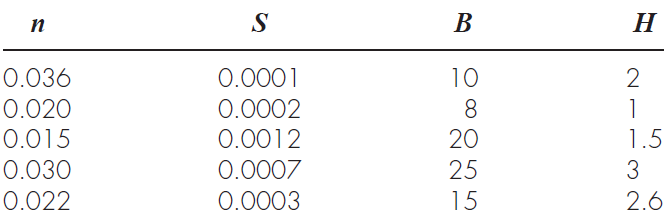
\includegraphics[width=0.9\linewidth]{./images/problem_3_3_8}
    \end{minipage}

    \noindent
    Write an M-file that computes the velocity for each of these
    channels. Enter these values into a matrix where each column
    represents a parameter and each row represents a channel.
    Have the M-file display the input data along with
    the computed velocity in tabular form where velocity is the
    fifth column. Include headings on the table to label the
    columns.\\

    \noindent\textbf{3.10} A simply supported beam is loaded as shown in
    Fig. P3.10. Using singularity functions, the displacement
    along the beam can be expressed by the equation:\\

    $u_y(x) = \dfrac{-5}{6}[\left\langle x - 0 \right\rangle^4 - \left\langle x-5 \right\rangle^4]
    +\dfrac{15}{6} \left\langle x-8 \right\rangle^3 +75\left\langle x-7 \right\rangle^2
    +\dfrac{57}{6}x^3 - 238.25x$\\

    \noindent By definition, the singularity function can be expressed as
    follows:\\

    $\langle x-a\rangle^{n}=\left\{\begin{array}{cc}
        (x-a)^{n} & \text{when } x>a \\
        0 & \text {when } x\leq a
        \end{array}\right\}$

    \noindent Develop an M-file that creates a plot of displacement
    (dashed line) versus distance along the beam, $x$. Note that
    $x = 0$ at the left end of the beam.\\

    \noindent\textbf{3.11} The volume $V$ of liquid in a hollow horizontal cylinder of
    radius $r$ and length $L$ is related to the depth of the liquid $h$ by\\

    $V = \Big[r^2cos^{-1}\Big(\dfrac{r-h}{r}-(r-h)\sqrt{2rh-h^2} \Big) \Big]L$\\

    \noindent Develop an M-file to create a plot of volume versus depth.
    Here are the first few lines:\\
    

   \texttt{\noindent function cylinder(r, L, plot\_title)\\
    \indent\% volume of horizontal cylinder\\
    \indent\% inputs:\\
    \indent\% r = radius\\
    \indent\% L = length\\
    \indent\% plot\_title = string holding\\
    \indent\hspace{40mm}plot title}\\

    \noindent Test your program with\\

    \texttt{\noindent>> cylinder(3,5,...\\
    \indent'Volume versus depth for...\\
    \indent horizontal cylindrical tank')}\\
    
    \noindent\textbf{3.12} Develop a vectorized version of the following code:\\

    \texttt{\noindent tstart=0; tend=20; ni=8;\\
    \indent t(1)=tstart;\\
    \indent y(1)=12 + 6*cos(2*pi*t(1)/...
    \indent\hspace{25mm}(tend-tstart));\\
    \indent for i=2:ni+1\\
    \indent\hspace{2mm} t(i)=t(i-1)+(tend-tstart)/ni;\\
    \indent\hspace{2mm} y(i)=10 + 5*cos(2*pi*t(i)/ ...\\
    \indent\hspace{25mm} (tend-tstart));\\
    \indent end}\\

    \noindent\textbf{3.13} The "divide and average" method, an old-time method
    for approximating the square root of any positive number $a$,
    can be formulated as\\

    $x = \dfrac{x+a/x}{2}$\\

    \noindent
    Write a well-structured M-file function based on the
    \texttt{while...break} loop structure to implement this algorithm.
    Use proper indentation so that the structure is clear. At
    each step estimate the error in your approximation as\\

    $\epsilon = \left\lvert \dfrac{x_{new} - x_{old}}{x_{new}} \right\rvert $\\

    \noindent
    Repeat the loop until $\epsilon$ is less than or equal to a specified
    value. Design your program so that it returns both the result
    and the error. Make sure that it can evaluate the square root
    of numbers that are equal to and less than zero. For the latter
    case, display the result as an imaginary number. For example,
    the square root of -4 would return $2i$. Test your program
    by evaluating $a = 0$, 2, 10 and -4 for $\epsilon = 1 \times 10^{-4}$.\\

    \noindent\textbf{3.14} \emph{Piecewise functions} are sometimes useful when the relationship
    between a dependent and an independent variable
    cannot be adequately represented by a single equation. For
    example, the velocity of a rocket might be described by\\

    $v(t)=\left\{\begin{array}{cc}
        10 t^{2}-5 t & 0 \leq t \leq 8 \\
        624-5 t & 8 \leq t \leq 16 \\
        36 t+12(t-16)^{2} & 16 \leq t \leq 26 \\
        2136 e^{-0.1(t-26)} & t>26 \\
        0 & \text { otherwise }
        \end{array}\right.$\\

    \noindent Develop an M-file function to compute $v$ as a function of t.
    Then, develop a script that uses this function to generate a
    plot of $v$ versus $t$ for $t=-5$ to 50.\\

    \noindent\textbf{3.15} Develop an M-file function called \texttt{rounder} to round a
    number x to a specified number of decimal digits, $n$. The first
    line of the function should be set up as\\

    \texttt{function xr = rounder(x, n)}\\

    \noindent Test the program by rounding each of the following to 2 decimal
    digits: x = 477.9587, -477.9587, 0.125, 0.135, -0.125,
    and -0.135.\\

    \noindent\textbf{3.16} Develop an M-file function to determine the elapsed
    days in a year. The first line of the function should be set
    up as\\

    \texttt{function nd = days(mo, da, leap)}\\

    \noindent where \texttt{mo} = the month (1-12), \texttt{da} = the day (1-31), and
    \texttt{leap} = (0 for non–leap year and 1 for leap year). Test it for
    January 1, 1997, February 29, 2004, March 1, 2001, June 21,
    2004, and December 31, 2008. Hint: A nice way to do this
    combines the \texttt{for} and the \texttt{switch} structures.\\

    \noindent\textbf{3.17} Develop an M-file function to determine the elapsed
    days in a year. The first line of the function should be set up as\\

    \texttt{function nd = days(mo, da, year)}\\

    \noindent where \texttt{mo} = the month (1-12), \texttt{da} = the day (1-31), and
    \texttt{year} = the year. Test it for January 1, 1997, February 29,
    2004, March 1, 2001, June 21, 2004, and December 31, 2008.\\

    \noindent\textbf{3.18} Develop a function function M-file that returns the difference
    between the passed function's maximum and minimum
    value given a range of the independent variable. In
    addition, have the function generate a plot of the function for
    the range. Test it for the following cases:\\

    \noindent
    \textbf{(a)} $f(t)=8e^{-0.25t}sin(t-2)$ from $t=0$ to $6\pi$\\
    \textbf{(b)} $f(x)=e^{4x}sin(1/x)$ from $x=0.01$ to $0.2$.\\
    \textbf{(c)} The built-in \texttt{humps} function from $x=0$ to 2.\\

    \noindent\textbf{3.19} Modify the function function \texttt{odesimp} developed at
    the end of Sec. 3.6 so that it can be passed the arguments of
    the passed function. Test it for the following case:\\

    \texttt{>> dvdt=@(v,m,cd) 9.81-(cd/m)*v\textasciicircum2;\\
    \indent >> odesimp(dvdt,0.5,0,12,\\
    \indent\hspace{40mm}-10,70,0.23)}\\

    \noindent\textbf{3.20} A Cartesian vector can be thought of as representing
    magnitudes along the $x$-, $y$-, and $z$-axes multiplied by a unit
    vector ($i$, $j$, $k$). For such cases, the dot product of two of these
    vectors \{$a$\} and \{$b$\} corresponds to the product of their magnitudes
    and the cosine of the angle between their tails as in\\

    $\{a\}\cdot \{b\} = abcos\theta$\\

    \noindent The cross product yields another vector, $\{c\} = \{a\} \times \{b\}$,
    which is perpendicular to the plane defined by $\{a\}$ and $\{b\}$
    such that its direction is specified by the right-hand rule.
    Develop an M-file function that is passed two such vectors
    and returns $\theta$, $\{c\}$ and the magnitude of $\{c\}$, and generates a
    three-dimensional plot of the three vectors $\{a\}$, $\{b\}$, and $\{c\}$
    with their origins at zero. Use dashed lines for $\{a\}$ and $\{b\}$
    and a solid line for $\{c\}$. Test your function for the following
    cases:\\

    \noindent
    \textbf{(a)} \texttt{a = [6 4 2]; b = [2 6 4];}\\
    \textbf{(b)} \texttt{a = [3 2 -6]; b = [4 -3 1];}\\
    \textbf{(c)} \texttt{a = [2 -2 1]; b = [4 2 -4];}\\
    \textbf{(d)} \texttt{a = [-1 0 0]; b = [0 -1 0];}\\

    \noindent\textbf{3.21} Based on Example 3.6, develop a script to produce an
    animation of a bouncing ball where $v_0$ = 5 m/s and $\theta_0 = 50^{\circ}$.
    To do this, you must be able to predict exactly when the ball
    hits the ground. At this point, the direction changes (the new
    angle will equal the negative of the angle at impact), and the
    velocity will decrease in magnitude to reflect energy loss
    due to the collision of the ball with the ground. The change
    in velocity can be quantified by the \emph{coefficient of restitution}
    $C_R$ which is equal to the ratio of the velocity after to the velocity
    before impact. For the present case, use a value of
    $C_R$ = 0.8.\\

    \noindent\textbf{3.22} Develop a function to produce an animation of a particle
    moving in a circle in Cartesian coordinates based on radial
    coordinates. Assume a constant radius, $r$, and allow the
    angle, $\theta$, to increase from zero to $2\pi$ in equal increments.
    The function's first lines should be\\

    \texttt{function phasor(r, nt, nm)\\
    \indent \% function to show the orbit of
    \indent\hspace{40mm} a phasor\\
    \indent \% r = radius\\
    \indent \% nt = number of increments for 
    \indent\hspace{50mm}theta\\
    \indent \% nm = number of movies}\\

    \noindent Test your function with\\

    \texttt{phasor(1, 256, 10)}\\

    \noindent\textbf{3.23} Develop a script to produce a movie for the butterfly
    plot from Prob. 2.22. Use a particle located at the $x$-$y$ coordinates
    to visualize how the plot evolves in time.
\end{multicols}

\end{document}





